
 \FloatBarrier

\section{Example: Demand response programs}\label{sec:dr_example}

This is an example of multiple populations used to implement demand response programs in smart grids \cite{barreto2013design, barreto2014incentives}. In this case, we assume that each user must decide how to distribute its electricity usage along a day. Particularly, 
agents might have conflicting interests because they might impose externalities on the society through the price signals, i.e., the aggregated demand might affect the profit of agents. This conflict can be seen as a game between agents, in which each agent is selfish and  endeavors to maximize independently its own welfare. 

In this problem we model the daily electricity allocation problem as a multi-population game with nonlinear fitness functions. Particularly, each agent can implement an evolutionary dynamic to find the best distribution of resources. Note that when implemented locally by each user, the evolutionary dynamics lead to the global efficient equilibrium (In this case the fitness is equal to the marginal utility of each agent). 

A particular feature of this problem is that the Nash equilibrium of the system is inefficient. Hence, 
we introduce an incentives scheme (indirect revelation mechanism) to maximize the aggregated surplus of the population.
The main feature of this mechanism is that it does not require private information from users, and employs a one dimensional message space to coordinate the demand profile of agents. These properties facilitate the distributed implementation of the mechanism. The mechanism entrusts the computation tasks among users, who should maximize its own utility function based the aggregated demand (that is calculated and broadcasted by a central agent). Thus, users avoid revelation of private information (e.g., preferences), but are required to report the aggregated consumption of their appliances during some time periods.







\subsubsection{Problem Formulation}



We consider a population composed by $N$ consumers defined as $\mathcal{V} = {1,\ldots.N}$. Also, let us divide a period of 24 hours in a set of $T$ time intervals denoted $\tau = \{\tau_1,\ldots,\tau_T\}$.
Formally, we define the set $\tau$ as a partition of $[0,24)$, where 
 $\cup_{t\in\{1,\ldots,T\}} \tau_t = \tau$ and $\cap_{t\in\{1,\ldots,T\}} \tau_t = \varnothing$.
%
Let $q_i^t$ be the electricity consumption of the $i\th$ user in the $t\th$ time interval. 
The daily electricity consumption of the $i\th$ user is represented by the vector $\bs{q}_i=[q_i^1,\ldots,q_i^T]^\top\in \Re_{\geq 0}^{T}$.
The population consumption at a given time $t$ is defined by the vector $\bs{q}^t = [q_1^t,, q_2^t\ldots,q_N^t]^\top\in \Re_{\geq 0}^{N}$.
On the other hand, the joint electricity consumption of the whole population is denoted by $\bs{q} = [\bs{q}_1^\top,
\ldots, \bs{q}_N^\top]^\top$. 
Without loss of generality, we assume that the electricity consumption of the $i\th$ user  satisfies $q_i^t\geq 0$,  in each time instant $t$.
A \emph{valuation function} $v_i^t(q_i^t)$ models the \emph{valuation} that the $i\th$ user gives to an electricity consumption of $q_i^t$ units in the $t\th$ time interval. Finally, let $p(\cdot):\Re\rightarrow\Re$ be the price of electricity charged to consumers. The aggregated consumption at a given time $t$ is defined as $||\bs{q}^t||_1 = \sum_{j=1}^N q_j^t$.
Moreover, a daily valuation is 
$v_i(\bs{q}_i)=\sum_{t=1}^T v_i^t(q_i^t),$
 where $t\in\{1,\ldots,T\}$.


 
 
 
Now, assuming  that the electricity generation cost is  the same for all $t$, we can express the profit function of each individual as
%
\begin{equation}\label{eq:u_i_}
 U_i(\bs{q}) = v_i(\bs{q}_i) - \sum_{t=1}^T q_i^t p\Big( \norm{\bs{q}^t}_1 \Big),
\end{equation}
%
where 
$p:\Re_+ \to \Re_+$ is the unitary price function.
The consumers welfare function is maximized by solving \cite{Johari09}
%
\begin{equation}\label{eq:opt_problem}
\begin{aligned}
& \underset{\bs{q}}{\text{maximize}}
& &  \sum_{i=1}^N U_i(\bs{q}) =  \sum_{i=1}^N\left( v_i(\bs{q}_i) - \sum_{t=1}^T q_i^t p\left( \norm{\bs{q}^t}_1 \right) \right) \\
& \text{subject to}
& & q_i^t \geq 0,  i =\{1,\ldots,N\}, t =\{1,\ldots,T\}.
\end{aligned}
\end{equation}



\subsubsection{Incentives}

The solution of the optimization problem in Eq.~(\ref{eq:opt_problem}) is inefficient in a strategic environment, i.e., when individuals are rational and selfish \cite{barreto2013design, Johari09}. In such cases, the analysis of strategic interactions among rational agents is made using game theory \cite{fudenberg98}.
In particular, the Nash equilibrium (a solution concept in game theory)  is sub-optimal, however, we can show that if we consider an added incentive to the individual cost function of each player, the Nash equilibrium of the game with incentives can be made efficient in the sense of Pareto \cite{barreto2013design, barreto2014incentives}. 

In particular, our DR scheme with incentives models the case when all agents keep their valuation of electricity to themselves, and have autonomous control their consumption. However, in order to incentive the agents to modify their behavior for the good of the population, the central entity sends them an incentive (e.g., a price signal or reward) to indirectly control their load.

Consider the new cost function for the $i^{th}$ agent:
\begin{equation}\label{eq:game2}
W_i(q_i,\bs{q}_{-i}) 
= v_i(q_i) -  q_i p\left( \norm{\bs{q}^t}_1 \right) + I_i(\bs{q}) .
\end{equation}
where incentives are of the form:
\begin{equation}\label{eq:I_i}
I_i(\bs{q}) = \left( \norm{\bs{q}_{-i}^t}_1\right) \left( h_i(\norm{\bs{q}_{-i}})  - p\left( \norm{\bs{q}^t}_1 \right) \right).
\end{equation}


The form of this incentive is inspired in the 
Vickrey-Clarke-Groves mechanism and the  Clarke pivot rule \cite{AlgorithmicG}.
%
We assign incentives according to the contribution made by an agent 
to the society. In particular, the function $h_i:\Re \to \Re$ is a design parameter that estimates the externalities introduced by each individual.
It can be shown that these incentives can lead to an optimal equilibrium in a strategic environment.
In this DR approach we consider that the utility sends a two dimensional signal to each customer, namely $(q,I_i)$ and each customer responds with some consumption $q_i$. 
Note that the incentives modify the price paid by each user according to their relative consumption. However, two different users receive different incentives as long as their consumption are different.





\subsubsection{Simulations}

In this section, we illustrate some ideas of efficiency and the decentralized implementation of the incentives mechanism. We select some functions used previously in the literature. On the one hand, we define the family of valuation functions as 
\begin{equation}\label{eq:valuation_sim}
 v(\bs{q}^k,\alpha_i^k) = v_i^k (q_i^k) = \alpha_i^k \log(1+q_i^k)
\end{equation}
where $\alpha_i^k>0$ is the parameter that characterizes the valuation of the  $i\th$ agent at the $k\th$ time instant.
On the other hand, the generation cost function is defined as 
%
\begin{equation}\label{eq:cost_sim}
 C(\|\bs{q}\|_1) = \beta ({\|\bs{q}\|_1})^2 + b {\|\bs{q}\|_1},
\end{equation}
and the unitary price function is
%
\begin{equation}\label{eq:p_sim}
 p(\|\bs{q}\|_1) = \frac{C(\|\bs{q}\|_1)}{\|\bs{q}\|_1} = \beta \|\bs{q}\|_1 + b.
\end{equation}
%
Note that the generation cost only depends on the aggregated consumption, not on the time of the day. Furthermore, 
%
the fitness function of the system with incentives is
%
\begin{equation}\label{eq:fitness_without_i_sim}
F_i^k( \bs{q}^k)  =  \frac{\alpha_i^k }{1+q_i^k}
 - 2\beta \left( \sum_{j=1}^N q_j^k  \right).
 \end{equation}


The evolution of utility, demand, and incentives for different dynamics is shown in Figs.~\ref{fig:dynamics_u} and \ref{fig:dynamics_i}. Note that despite using the same initial condition, the evolution of the system is different with each dynamical model. In particular, BNN and Smith dynamics converge faster to the  optimum, in contrast with the Logit and replicator dynamics. 
This is achieved by means of a fast decrease in the power consumption. 

\begin{figure}[hbt]
 \centering
 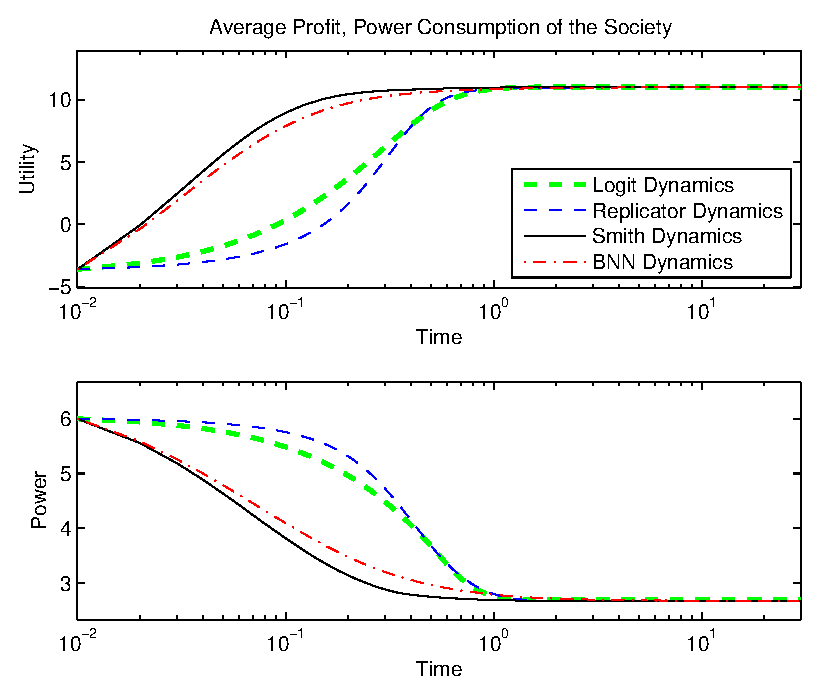
\includegraphics[width=.75\textwidth]{./images/evolution_u.eps}
 \caption{Evolution of profit and costs for four different dynamics.}
 \label{fig:dynamics_u}
\end{figure}


\begin{figure}[hbt]
 \centering
 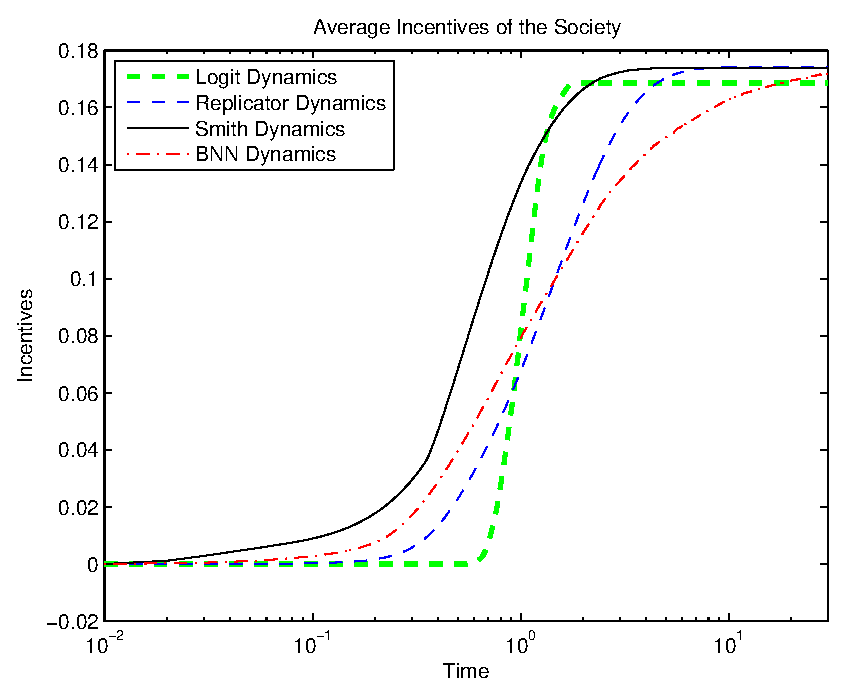
\includegraphics[width=.75\textwidth]{./images/evolution_i.eps}
 \caption{Evolution of the incentives with four different dynamics.}
 \label{fig:dynamics_i}
\end{figure}



Incentives in Fig.~\ref{fig:dynamics_i} show that, in the long run, all dynamics converge to the same level of incentives. Particularly, Smith dynamics requires more incentives during all time, except for logit dynamics, which has a sudden increase in the incentives close to the equilibrium point. 

In Fig.~\ref{fig:dynamics_i} it is not clear which dynamical model moves the state of the system to the optimal equilibrium using less resources. To answer this question, we simulate the total amount of incentives used by each model.
Thus, let us define the aggregated incentives in a society in a particular time $t$ as
\begin{equation}
 I_d (t) = \sum_{i\in\mathcal{P}} \frac{1}{|S|} \sum_{k\in S} I_i \left( \bs{q}^k (t) \right).
\end{equation}
Now, the total accumulated incentives from $t_0$ to $t$ is defined as 
\begin{equation}
 \varPhi_d (t) = \int_{t_0}^t I_d (\tau) d\tau.
\end{equation}
Thus, $\varPhi_d (t)$ gives a measurement of the total amount subsidies required by the system with dynamic $d$, in the time interval  $[t_0, t]$.
In this case we do not have a reference to compare the subsidies requirements of each evolutionary dynamic. Hence, we compare the subsidies requirements with the average requirements of all the dynamics implemented. 
%
In order to see which dynamic requires more resources, we plot the cumulative resources required by each dynamic relative to the average.
Hence, we define the cumulative incentives as 
%
\begin{equation}
CI_d = \frac{ \varPhi_d (t) }{ \sum_{d\in \mathcal{D}} \varPhi_d (t) }.
\end{equation}
%
Fig.~\ref{fig:integral} shows the results of the simulation of the relative subsidies required by each model of evolutionary dynamics.
%



Smith dynamics requires much more resources during all the time stamp, but is particularly high during the first stages, while logit has the lower incentives requirements. However, BNN has the lower incentives in long run.

\begin{figure}[hbt]
 \centering
 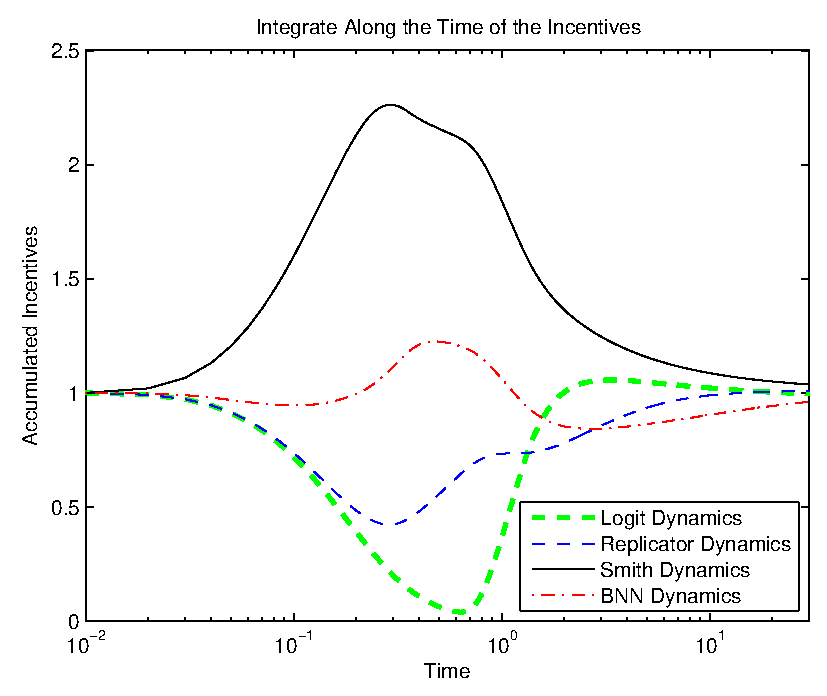
\includegraphics[width=.75\textwidth]{./images/accumulated_i.eps}
 \caption{Accumulated incentives during the evolution of the algorithm.}
 \label{fig:integral}
\end{figure}



Fig. \ref{fig:final_state} shows the final demand profile of each agent. Note that the final state corresponds to the state of each population at the equilibrium.

\begin{figure}[hbt]
 \centering
 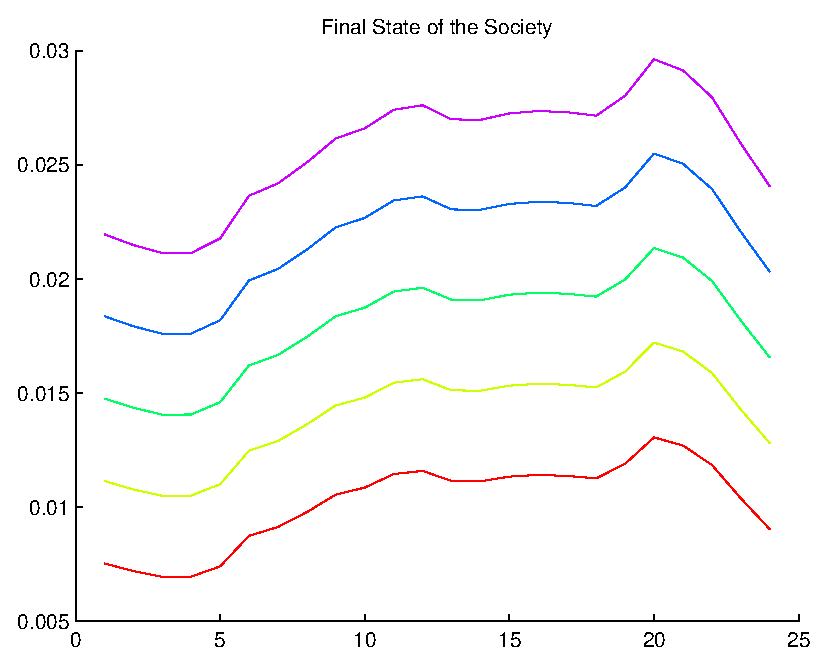
\includegraphics[width=.75\textwidth]{./images/final_state.eps}
 \caption{Final demand profile of each agent.}
 \label{fig:final_state}
\end{figure}
